\documentclass[twoside]{book}

% Packages required by doxygen
\usepackage{fixltx2e}
\usepackage{calc}
\usepackage{doxygen}
\usepackage[export]{adjustbox} % also loads graphicx
\usepackage{graphicx}
\usepackage[utf8]{inputenc}
\usepackage{makeidx}
\usepackage{multicol}
\usepackage{multirow}
\PassOptionsToPackage{warn}{textcomp}
\usepackage{textcomp}
\usepackage[nointegrals]{wasysym}
\usepackage[table]{xcolor}

% Font selection
\usepackage[T1]{fontenc}
\usepackage[scaled=.90]{helvet}
\usepackage{courier}
\usepackage{amssymb}
\usepackage{sectsty}
\renewcommand{\familydefault}{\sfdefault}
\allsectionsfont{%
  \fontseries{bc}\selectfont%
  \color{darkgray}%
}
\renewcommand{\DoxyLabelFont}{%
  \fontseries{bc}\selectfont%
  \color{darkgray}%
}
\newcommand{\+}{\discretionary{\mbox{\scriptsize$\hookleftarrow$}}{}{}}

% Page & text layout
\usepackage{geometry}
\geometry{%
  a4paper,%
  top=2.5cm,%
  bottom=2.5cm,%
  left=2.5cm,%
  right=2.5cm%
}
\tolerance=750
\hfuzz=15pt
\hbadness=750
\setlength{\emergencystretch}{15pt}
\setlength{\parindent}{0cm}
\setlength{\parskip}{3ex plus 2ex minus 2ex}
\makeatletter
\renewcommand{\paragraph}{%
  \@startsection{paragraph}{4}{0ex}{-1.0ex}{1.0ex}{%
    \normalfont\normalsize\bfseries\SS@parafont%
  }%
}
\renewcommand{\subparagraph}{%
  \@startsection{subparagraph}{5}{0ex}{-1.0ex}{1.0ex}{%
    \normalfont\normalsize\bfseries\SS@subparafont%
  }%
}
\makeatother

% Headers & footers
\usepackage{fancyhdr}
\pagestyle{fancyplain}
\fancyhead[LE]{\fancyplain{}{\bfseries\thepage}}
\fancyhead[CE]{\fancyplain{}{}}
\fancyhead[RE]{\fancyplain{}{\bfseries\leftmark}}
\fancyhead[LO]{\fancyplain{}{\bfseries\rightmark}}
\fancyhead[CO]{\fancyplain{}{}}
\fancyhead[RO]{\fancyplain{}{\bfseries\thepage}}
\fancyfoot[LE]{\fancyplain{}{}}
\fancyfoot[CE]{\fancyplain{}{}}
\fancyfoot[RE]{\fancyplain{}{\bfseries\scriptsize Generated by Doxygen }}
\fancyfoot[LO]{\fancyplain{}{\bfseries\scriptsize Generated by Doxygen }}
\fancyfoot[CO]{\fancyplain{}{}}
\fancyfoot[RO]{\fancyplain{}{}}
\renewcommand{\footrulewidth}{0.4pt}
\renewcommand{\chaptermark}[1]{%
  \markboth{#1}{}%
}
\renewcommand{\sectionmark}[1]{%
  \markright{\thesection\ #1}%
}

% Indices & bibliography
\usepackage{natbib}
\usepackage[titles]{tocloft}
\setcounter{tocdepth}{3}
\setcounter{secnumdepth}{5}
\makeindex

% Hyperlinks (required, but should be loaded last)
\usepackage{ifpdf}
\ifpdf
  \usepackage[pdftex,pagebackref=true]{hyperref}
\else
  \usepackage[ps2pdf,pagebackref=true]{hyperref}
\fi
\hypersetup{%
  colorlinks=true,%
  linkcolor=blue,%
  citecolor=blue,%
  unicode%
}

% Custom commands
\newcommand{\clearemptydoublepage}{%
  \newpage{\pagestyle{empty}\cleardoublepage}%
}

\usepackage{caption}
\captionsetup{labelsep=space,justification=centering,font={bf},singlelinecheck=off,skip=4pt,position=top}

%===== C O N T E N T S =====

\begin{document}

% Titlepage & ToC
\hypersetup{pageanchor=false,
             bookmarksnumbered=true,
             pdfencoding=unicode
            }
\pagenumbering{alph}
\begin{titlepage}
\vspace*{7cm}
\begin{center}%
{\Large E\+E513 -\/ Connected Embedded Systems\+: Assignment 1 }\\
\vspace*{1cm}
{\large Generated by Doxygen 1.8.13}\\
\end{center}
\end{titlepage}
\clearemptydoublepage
\pagenumbering{roman}
\tableofcontents
\clearemptydoublepage
\pagenumbering{arabic}
\hypersetup{pageanchor=true}

%--- Begin generated contents ---
\chapter{E\+E513 -\/ Connected Embedded Systems\+: Assignment 1}
\label{md_README}
\Hypertarget{md_README}
This assignment focuses on interfacing a \hyperlink{classDS3231}{D\+S3231} R\+TC with an embedded linux device -\/ in my case, a Raspberry Pi 3 B+. 
\chapter{Hierarchical Index}
\section{Class Hierarchy}
This inheritance list is sorted roughly, but not completely, alphabetically\+:\begin{DoxyCompactList}
\item \contentsline{section}{I2\+C\+Device}{\pageref{classI2CDevice}}{}
\begin{DoxyCompactList}
\item \contentsline{section}{D\+S3231}{\pageref{classDS3231}}{}
\end{DoxyCompactList}
\end{DoxyCompactList}

\chapter{Class Index}
\section{Class List}
Here are the classes, structs, unions and interfaces with brief descriptions\+:\begin{DoxyCompactList}
\item\contentsline{section}{\hyperlink{classDS3231}{D\+S3231} }{\pageref{classDS3231}}{}
\item\contentsline{section}{\hyperlink{classI2CDevice}{I2\+C\+Device} }{\pageref{classI2CDevice}}{}
\end{DoxyCompactList}

\chapter{Class Documentation}
\hypertarget{classDS3231}{}\section{D\+S3231 Class Reference}
\label{classDS3231}\index{D\+S3231@{D\+S3231}}


Inheritance diagram for D\+S3231\+:
\nopagebreak
\begin{figure}[H]
\begin{center}
\leavevmode
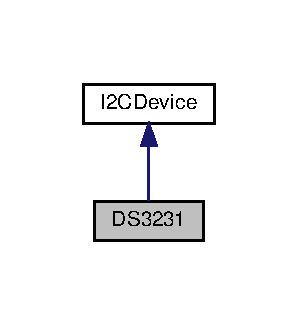
\includegraphics[width=143pt]{classDS3231__inherit__graph}
\end{center}
\end{figure}


Collaboration diagram for D\+S3231\+:
\nopagebreak
\begin{figure}[H]
\begin{center}
\leavevmode
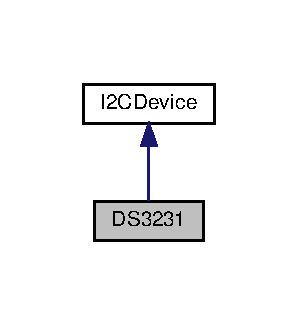
\includegraphics[width=143pt]{classDS3231__coll__graph}
\end{center}
\end{figure}
\subsection*{Public Member Functions}
\begin{DoxyCompactItemize}
\item 
\mbox{\Hypertarget{classDS3231_a35b7baeaa8c8449c0c08b37a7ef0f21b}\label{classDS3231_a35b7baeaa8c8449c0c08b37a7ef0f21b}} 
{\bfseries D\+S3231} (char)
\item 
\mbox{\Hypertarget{classDS3231_acdbdfefb5bd96582ef46703a375a96e6}\label{classDS3231_acdbdfefb5bd96582ef46703a375a96e6}} 
{\bfseries D\+S3231} (bool)
\item 
void \hyperlink{classDS3231_ae7630e2f75c91d116f503292163fc2e9}{sys\+Time\+R\+T\+C\+Init} ()
\item 
void \hyperlink{classDS3231_a847c85a36bf3ab13c942b91733bbbe24}{read\+Time\+And\+Date} ()
\item 
void \hyperlink{classDS3231_a8780408536a9eedfe2f04d4085a103b0}{write\+Time} (char $\ast$)
\item 
void \hyperlink{classDS3231_aa8b6b1279d7f7e04cd4a3797d620cf61}{write\+Date} (char $\ast$)
\item 
void \hyperlink{classDS3231_aee6cdb9ddbce1c2efe76d50cd042fb08}{read\+Alarms} ()
\item 
void \hyperlink{classDS3231_a78d2a067addcb2b5a43962e6442ca060}{set\+Alarms} (char $\ast$)
\item 
void \hyperlink{classDS3231_a9529ddedfae9e6e427197c26ac7c8f0b}{read\+Temp} ()
\item 
void \hyperlink{classDS3231_a43d0b34f3adb3abd8529ccafb23b3c66}{set\+Interrupt} (bool, bool)
\item 
void \hyperlink{classDS3231_a0a56ae678b3708a07e3d8878774b42a8}{sq\+Wave\+Gen} (int, bool)
\item 
void \hyperlink{classDS3231_ad402ba1ca960dd1d1da5fc68d806696e}{clear\+Alarms} ()
\end{DoxyCompactItemize}
\subsection*{Additional Inherited Members}


\subsection{Member Function Documentation}
\mbox{\Hypertarget{classDS3231_ad402ba1ca960dd1d1da5fc68d806696e}\label{classDS3231_ad402ba1ca960dd1d1da5fc68d806696e}} 
\index{D\+S3231@{D\+S3231}!clear\+Alarms@{clear\+Alarms}}
\index{clear\+Alarms@{clear\+Alarms}!D\+S3231@{D\+S3231}}
\subsubsection{\texorpdfstring{clear\+Alarms()}{clearAlarms()}}
{\footnotesize\ttfamily void D\+S3231\+::clear\+Alarms (\begin{DoxyParamCaption}{ }\end{DoxyParamCaption})}

Clear the R\+TC Alarm Flags

Clears the Alarm 1 and Alarm 2 Flag bits of register 0x0F.\mbox{\Hypertarget{classDS3231_aee6cdb9ddbce1c2efe76d50cd042fb08}\label{classDS3231_aee6cdb9ddbce1c2efe76d50cd042fb08}} 
\index{D\+S3231@{D\+S3231}!read\+Alarms@{read\+Alarms}}
\index{read\+Alarms@{read\+Alarms}!D\+S3231@{D\+S3231}}
\subsubsection{\texorpdfstring{read\+Alarms()}{readAlarms()}}
{\footnotesize\ttfamily void D\+S3231\+::read\+Alarms (\begin{DoxyParamCaption}{ }\end{DoxyParamCaption})}

Print the R\+TC Alarms

Prints the values stored in the Alarm 1 and Alarm 2 registers (0x07 -\/ 0x0D).\mbox{\Hypertarget{classDS3231_a9529ddedfae9e6e427197c26ac7c8f0b}\label{classDS3231_a9529ddedfae9e6e427197c26ac7c8f0b}} 
\index{D\+S3231@{D\+S3231}!read\+Temp@{read\+Temp}}
\index{read\+Temp@{read\+Temp}!D\+S3231@{D\+S3231}}
\subsubsection{\texorpdfstring{read\+Temp()}{readTemp()}}
{\footnotesize\ttfamily void D\+S3231\+::read\+Temp (\begin{DoxyParamCaption}{ }\end{DoxyParamCaption})}

Print the R\+TC temperature

Temperature has a precision of 0.\+25 degrees. The upper part of the temperature is in reg 1 The lower part of the temperature is in tbe upper two bits of reg 2\mbox{\Hypertarget{classDS3231_a847c85a36bf3ab13c942b91733bbbe24}\label{classDS3231_a847c85a36bf3ab13c942b91733bbbe24}} 
\index{D\+S3231@{D\+S3231}!read\+Time\+And\+Date@{read\+Time\+And\+Date}}
\index{read\+Time\+And\+Date@{read\+Time\+And\+Date}!D\+S3231@{D\+S3231}}
\subsubsection{\texorpdfstring{read\+Time\+And\+Date()}{readTimeAndDate()}}
{\footnotesize\ttfamily void D\+S3231\+::read\+Time\+And\+Date (\begin{DoxyParamCaption}{ }\end{DoxyParamCaption})}

Print the R\+TC Time and Date

Prints the values stored in registers 2, 1, and 0 (Hours, Minutes, Seconds), followed by registers 3, 4, 5, and 6 ( Day, Date, Month, Year).\mbox{\Hypertarget{classDS3231_a78d2a067addcb2b5a43962e6442ca060}\label{classDS3231_a78d2a067addcb2b5a43962e6442ca060}} 
\index{D\+S3231@{D\+S3231}!set\+Alarms@{set\+Alarms}}
\index{set\+Alarms@{set\+Alarms}!D\+S3231@{D\+S3231}}
\subsubsection{\texorpdfstring{set\+Alarms()}{setAlarms()}}
{\footnotesize\ttfamily void D\+S3231\+::set\+Alarms (\begin{DoxyParamCaption}\item[{char $\ast$}]{times }\end{DoxyParamCaption})}

Set the R\+TC Alarm Times/\+Dates

Writes to the Alarm registers (0x07 -\/ 0x0D). Sets all \char`\"{}\+Alarm Mask Bits\char`\"{} to 0 -\/ Alarm will trigger when date, hours, minutes and seconds match\mbox{\Hypertarget{classDS3231_a43d0b34f3adb3abd8529ccafb23b3c66}\label{classDS3231_a43d0b34f3adb3abd8529ccafb23b3c66}} 
\index{D\+S3231@{D\+S3231}!set\+Interrupt@{set\+Interrupt}}
\index{set\+Interrupt@{set\+Interrupt}!D\+S3231@{D\+S3231}}
\subsubsection{\texorpdfstring{set\+Interrupt()}{setInterrupt()}}
{\footnotesize\ttfamily void D\+S3231\+::set\+Interrupt (\begin{DoxyParamCaption}\item[{bool}]{alarm1,  }\item[{bool}]{alarm2 }\end{DoxyParamCaption})}

Set the R\+TC Alarm Interrupt

Takes two boolean values representing the status of alarms 1 and 2. If either are to be set, the interrupt is set, along with the corresponding alarm enable bit. If neither are set, the interrupt bit is cleared, i.\+e. the Square Wave Generator is enabled.\mbox{\Hypertarget{classDS3231_a0a56ae678b3708a07e3d8878774b42a8}\label{classDS3231_a0a56ae678b3708a07e3d8878774b42a8}} 
\index{D\+S3231@{D\+S3231}!sq\+Wave\+Gen@{sq\+Wave\+Gen}}
\index{sq\+Wave\+Gen@{sq\+Wave\+Gen}!D\+S3231@{D\+S3231}}
\subsubsection{\texorpdfstring{sq\+Wave\+Gen()}{sqWaveGen()}}
{\footnotesize\ttfamily void D\+S3231\+::sq\+Wave\+Gen (\begin{DoxyParamCaption}\item[{int}]{freq\+Option,  }\item[{bool}]{stop\+Interrupt }\end{DoxyParamCaption})}

Enable the Square Wave Generator at the desired frequency

Takes an integer value representing one of the four available frequencies of the square wave generator. A boolean represents the toggling of the interrupt bit, which enables the generator is set low. Each case of the switch statement performs the required bit modifications for the \char`\"{}\+Rate Select\char`\"{} bits of register 0x0E.\mbox{\Hypertarget{classDS3231_ae7630e2f75c91d116f503292163fc2e9}\label{classDS3231_ae7630e2f75c91d116f503292163fc2e9}} 
\index{D\+S3231@{D\+S3231}!sys\+Time\+R\+T\+C\+Init@{sys\+Time\+R\+T\+C\+Init}}
\index{sys\+Time\+R\+T\+C\+Init@{sys\+Time\+R\+T\+C\+Init}!D\+S3231@{D\+S3231}}
\subsubsection{\texorpdfstring{sys\+Time\+R\+T\+C\+Init()}{sysTimeRTCInit()}}
{\footnotesize\ttfamily void D\+S3231\+::sys\+Time\+R\+T\+C\+Init (\begin{DoxyParamCaption}{ }\end{DoxyParamCaption})}

Sets the R\+TC time based on the output of the Linux \char`\"{}date\char`\"{} utility.

This function creates a temporary file, runs the command line \char`\"{}date\char`\"{} utility -\/ formatting to give time (sec min hr) and date (day, date, month, year), and stores the output in the temporary file. This file is read into a string vector and the temporary file is closed and deleted. The time values and date values are added to separate char arrays for writing to the R\+TC.\mbox{\Hypertarget{classDS3231_aa8b6b1279d7f7e04cd4a3797d620cf61}\label{classDS3231_aa8b6b1279d7f7e04cd4a3797d620cf61}} 
\index{D\+S3231@{D\+S3231}!write\+Date@{write\+Date}}
\index{write\+Date@{write\+Date}!D\+S3231@{D\+S3231}}
\subsubsection{\texorpdfstring{write\+Date()}{writeDate()}}
{\footnotesize\ttfamily void D\+S3231\+::write\+Date (\begin{DoxyParamCaption}\item[{char $\ast$}]{date }\end{DoxyParamCaption})}

Write the input dates to the R\+TC date registers

Takes a character array containing \char`\"{}date\char`\"{} values to be written. Calls the \char`\"{}write\+To\+Reg\char`\"{} function to write the required value to the required registers. Defined values are used to reference the day, date, month. and year registers (0x03, 0x04, 0x05 and 0x06). A check is performed to ensure the date is within the correct range\mbox{\Hypertarget{classDS3231_a8780408536a9eedfe2f04d4085a103b0}\label{classDS3231_a8780408536a9eedfe2f04d4085a103b0}} 
\index{D\+S3231@{D\+S3231}!write\+Time@{write\+Time}}
\index{write\+Time@{write\+Time}!D\+S3231@{D\+S3231}}
\subsubsection{\texorpdfstring{write\+Time()}{writeTime()}}
{\footnotesize\ttfamily void D\+S3231\+::write\+Time (\begin{DoxyParamCaption}\item[{char $\ast$}]{times }\end{DoxyParamCaption})}

Write the input times to the R\+TC time registers

Takes a character array containing \char`\"{}time\char`\"{} values to be written. Calls the \char`\"{}write\+To\+Reg\char`\"{} function to write the required value to the required registers. Defined values are used to reference the second, minute and hour registers (0x00, 0x01, and 0x02).

The documentation for this class was generated from the following files\+:\begin{DoxyCompactItemize}
\item 
D\+S3231.\+h\item 
D\+S3231.\+cpp\end{DoxyCompactItemize}

\hypertarget{classI2CDevice}{}\section{I2\+C\+Device Class Reference}
\label{classI2CDevice}\index{I2\+C\+Device@{I2\+C\+Device}}


{\ttfamily \#include $<$I2\+C\+Device.\+h$>$}



Inheritance diagram for I2\+C\+Device\+:
\nopagebreak
\begin{figure}[H]
\begin{center}
\leavevmode
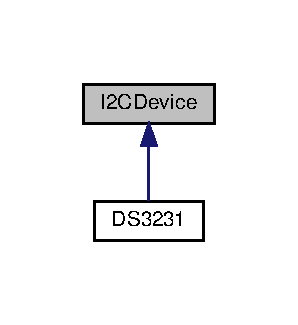
\includegraphics[width=143pt]{classI2CDevice__inherit__graph}
\end{center}
\end{figure}
\subsection*{Public Member Functions}
\begin{DoxyCompactItemize}
\item 
\mbox{\Hypertarget{classI2CDevice_a813e9eaaed2de0a6089e061e925f25a7}\label{classI2CDevice_a813e9eaaed2de0a6089e061e925f25a7}} 
{\bfseries I2\+C\+Device} (int)
\item 
\mbox{\Hypertarget{classI2CDevice_a5967d5f4321fdb12006f1d3892f050f8}\label{classI2CDevice_a5967d5f4321fdb12006f1d3892f050f8}} 
{\bfseries I2\+C\+Device} (int, char)
\end{DoxyCompactItemize}
\subsection*{Protected Member Functions}
\begin{DoxyCompactItemize}
\item 
int \hyperlink{classI2CDevice_a5fde7fd1a0060a67fc79508cadf6aace}{open\+Bus} ()
\item 
void \hyperlink{classI2CDevice_a97ce3e695080f667e4acfa4c6fe82ba4}{connect\+Device} ()
\item 
void \hyperlink{classI2CDevice_a683bdc938beaea0fc8af85f3996c4aa6}{reset\+Read\+Addr} ()
\item 
char $\ast$ \hyperlink{classI2CDevice_a46507a420f6865581ad41d6198897ee7}{read\+Buffer} ()
\item 
void \hyperlink{classI2CDevice_a390fcd7a411fbc92509a69c1d04660a2}{write\+To\+Reg} (unsigned int, char)
\item 
void \hyperlink{classI2CDevice_aa3a0bbea776167210f22dc03580757b1}{setup\+Proc} ()
\end{DoxyCompactItemize}
\subsection*{Protected Attributes}
\begin{DoxyCompactItemize}
\item 
\mbox{\Hypertarget{classI2CDevice_aab6762690a7288b436e408752fedc1ad}\label{classI2CDevice_aab6762690a7288b436e408752fedc1ad}} 
int {\bfseries file}
\item 
\mbox{\Hypertarget{classI2CDevice_a3c99b92a232fc4a7394e97caec29bddf}\label{classI2CDevice_a3c99b92a232fc4a7394e97caec29bddf}} 
std\+::vector$<$ char $>$ {\bfseries buf}
\item 
\mbox{\Hypertarget{classI2CDevice_a59a88fa7b1efd226ffd97c08fb5ece6a}\label{classI2CDevice_a59a88fa7b1efd226ffd97c08fb5ece6a}} 
char {\bfseries addr}
\end{DoxyCompactItemize}


\subsection{Detailed Description}
\hyperlink{classI2CDevice}{I2\+C\+Device} Class 

\subsection{Member Function Documentation}
\mbox{\Hypertarget{classI2CDevice_a97ce3e695080f667e4acfa4c6fe82ba4}\label{classI2CDevice_a97ce3e695080f667e4acfa4c6fe82ba4}} 
\index{I2\+C\+Device@{I2\+C\+Device}!connect\+Device@{connect\+Device}}
\index{connect\+Device@{connect\+Device}!I2\+C\+Device@{I2\+C\+Device}}
\subsubsection{\texorpdfstring{connect\+Device()}{connectDevice()}}
{\footnotesize\ttfamily void I2\+C\+Device\+::connect\+Device (\begin{DoxyParamCaption}{ }\end{DoxyParamCaption})\hspace{0.3cm}{\ttfamily [protected]}}

Open the connection to the I2C Device\mbox{\Hypertarget{classI2CDevice_a5fde7fd1a0060a67fc79508cadf6aace}\label{classI2CDevice_a5fde7fd1a0060a67fc79508cadf6aace}} 
\index{I2\+C\+Device@{I2\+C\+Device}!open\+Bus@{open\+Bus}}
\index{open\+Bus@{open\+Bus}!I2\+C\+Device@{I2\+C\+Device}}
\subsubsection{\texorpdfstring{open\+Bus()}{openBus()}}
{\footnotesize\ttfamily int I2\+C\+Device\+::open\+Bus (\begin{DoxyParamCaption}{ }\end{DoxyParamCaption})\hspace{0.3cm}{\ttfamily [protected]}}

Open the Bus connection to the I2C Device\mbox{\Hypertarget{classI2CDevice_a46507a420f6865581ad41d6198897ee7}\label{classI2CDevice_a46507a420f6865581ad41d6198897ee7}} 
\index{I2\+C\+Device@{I2\+C\+Device}!read\+Buffer@{read\+Buffer}}
\index{read\+Buffer@{read\+Buffer}!I2\+C\+Device@{I2\+C\+Device}}
\subsubsection{\texorpdfstring{read\+Buffer()}{readBuffer()}}
{\footnotesize\ttfamily char $\ast$ I2\+C\+Device\+::read\+Buffer (\begin{DoxyParamCaption}{ }\end{DoxyParamCaption})\hspace{0.3cm}{\ttfamily [protected]}}

Reads from the I2C devices registers\mbox{\Hypertarget{classI2CDevice_a683bdc938beaea0fc8af85f3996c4aa6}\label{classI2CDevice_a683bdc938beaea0fc8af85f3996c4aa6}} 
\index{I2\+C\+Device@{I2\+C\+Device}!reset\+Read\+Addr@{reset\+Read\+Addr}}
\index{reset\+Read\+Addr@{reset\+Read\+Addr}!I2\+C\+Device@{I2\+C\+Device}}
\subsubsection{\texorpdfstring{reset\+Read\+Addr()}{resetReadAddr()}}
{\footnotesize\ttfamily void I2\+C\+Device\+::reset\+Read\+Addr (\begin{DoxyParamCaption}{ }\end{DoxyParamCaption})\hspace{0.3cm}{\ttfamily [protected]}}

Set the initial read address for the I2C Device\mbox{\Hypertarget{classI2CDevice_aa3a0bbea776167210f22dc03580757b1}\label{classI2CDevice_aa3a0bbea776167210f22dc03580757b1}} 
\index{I2\+C\+Device@{I2\+C\+Device}!setup\+Proc@{setup\+Proc}}
\index{setup\+Proc@{setup\+Proc}!I2\+C\+Device@{I2\+C\+Device}}
\subsubsection{\texorpdfstring{setup\+Proc()}{setupProc()}}
{\footnotesize\ttfamily void I2\+C\+Device\+::setup\+Proc (\begin{DoxyParamCaption}{ }\end{DoxyParamCaption})\hspace{0.3cm}{\ttfamily [protected]}}

Setup Procedure for I2C Devices

Calls the functions required to open an I2C connection to a device, and read the buffers of this device.\mbox{\Hypertarget{classI2CDevice_a390fcd7a411fbc92509a69c1d04660a2}\label{classI2CDevice_a390fcd7a411fbc92509a69c1d04660a2}} 
\index{I2\+C\+Device@{I2\+C\+Device}!write\+To\+Reg@{write\+To\+Reg}}
\index{write\+To\+Reg@{write\+To\+Reg}!I2\+C\+Device@{I2\+C\+Device}}
\subsubsection{\texorpdfstring{write\+To\+Reg()}{writeToReg()}}
{\footnotesize\ttfamily void I2\+C\+Device\+::write\+To\+Reg (\begin{DoxyParamCaption}\item[{unsigned int}]{reg,  }\item[{char}]{val }\end{DoxyParamCaption})\hspace{0.3cm}{\ttfamily [protected]}}

Write to the I2C Devices registers

The documentation for this class was generated from the following files\+:\begin{DoxyCompactItemize}
\item 
I2\+C\+Device.\+h\item 
I2\+C\+Device.\+cpp\end{DoxyCompactItemize}

%--- End generated contents ---

% Index
\backmatter
\newpage
\phantomsection
\clearemptydoublepage
\addcontentsline{toc}{chapter}{Index}
\printindex

\end{document}
